\chapter{Τεχνικές Βαθιάς Μηχανικής Μάθησης και Αναγνώριση Αντικειμένωνν στον χώρο}
\label{chapter:theory}

%Στο κεφάλαιο αυτό, παρουσιάζεται και αναλύεται το θεωρητικό υπόβαθρο,
%στο οποίο στηρίχτηκαν οι υλοποιήσεις, στην παρούσα διπλωματική εργασία.

%Στο Κεφάλαιο \ref{sec:theory_ml}, παρουσιάζονται οι βασικές αρχές
%και τεχνικες \emph{Μηχανικής Μάθησης} (Machine Learning - ML).

Τα τελευταία χρόνια, ο κλάδος της Τεχνιτής Νοημοσύνης είναι ένας από τους πιο ραγδαία
αναπτυσσόμενους κλάδους της επιστήμης της πληροφορικής με τεράστιο
ερευνητικό και πρακτικό ενδιαφέρον; διαιρείται σε δύο υπο\_\_\_; την \emph{συμβολική τεχνιτή
νοημοσύνη} και την \emph{υποσυμβολική τεχνητή νοημοσύνη}. Η πρώτη προσπαθεί να
επιλύσει τα προβλήματα χρησιμοποιώντας αλγοριθμικές διαδικασίες, δηλαδή
σύμβολα και λογικούς κανόνες, ενώ η δεύτερη προσπαθεί να αναπαράγει την
ανθρώπινη "ευφυία" μέσα από την χρήση αριθμητικών μοντέλων
που με την σύνθεσή τους προσομοιώνουν την λειτουργία του ανθρώπινου εγκεφάλου
(υπολογιστική νοημοσύνη).
Η ικανότητα ενός νοούμενου (AI) συστήματος, να αποκτά από μόνο του γνώση,
εξάγοντας πρότυπα ή/και χαρακτηριστικά σημεία από τα δεδομένα,
είναι γνωστή ώς \emph{Μηχανική Μάθηση} (ML).
Η εισαγωγή του κλάδου του ML στην επιστήμη των υπολογιστών,
επέτρεψε στους υπολογιστές να μπορούν να αντιμετωπίσουν προβλήματα που εμπλέκουν
την αντίληψη για τον πραγματικό κόσμο και να πέρνουν υποκειμενικές αποφάσεις.
\begin{figure}[H]
  \centering
  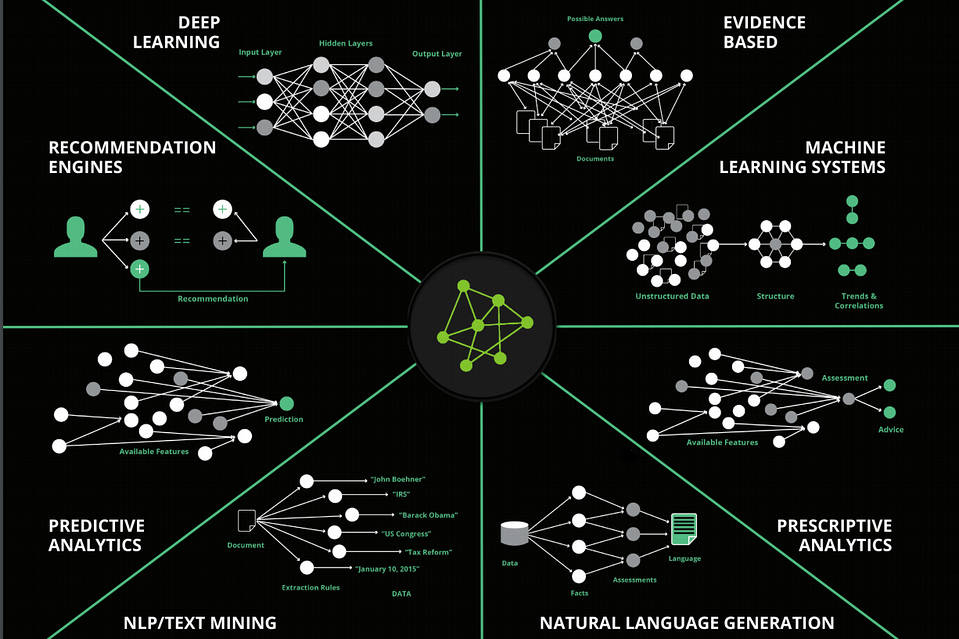
\includegraphics[width=0.9\textwidth]{./images/chapter3/AI_1.jpg}
  \caption[Τεχνητή Νοημοσύνη]{Τεχνητή Νοημοσύνη}
  \label{fig:AI_1}
\end{figure}
Η χρησιμοποίηση αλγορίθμων ML, επιτρέπουν σε συστήματα AI
να προσαρμόζονται εύκολα σε καινούργια έργα, με ελάχιστη επέμβαση από τον άνθρωπο.
Για παράδειγμα, ένα Νευρωνικό Δίκτυο που έχει εκπεδευτεί να αναγνωρίζει γάτους σε εικόνες,
δεν απαιτεί να σχεδιαστεί και να εκπαιδευτεί από το μηδέν για να έχει την ικανότητα
να αναγνωρίζει και σκύλους.

Πολλά προβλήματα, ενώ μέχρι και πριν μία μερικά χρόνια λύνονταν με
"χειρόγραφη", προγραμματισμένη από τον άνθρωπο γνώση, σήμερα χρησιμοποιούνται
αλγόριθμοι ML για την επίλυσή τους. Πιο κάτω παρατίθενται μερικά
παραδείγματα:
\begin{itemize}
  \item{Αναγνώριση ομιλίας - Speech Recognition}
  \item{Μηχανική όραση - Computer Vision}
  \begin{itemize}
    \item{Αναγνώριση αντικειμένων σε εικόνες - Object Recognition}
    \item{Αναγνώριση και εντοπισμός της θέσης αντικειμένων σε εικόνες - Object Detection}
  \end{itemize}
  \item{Αναγνώριση ηλεκτρονικών επιθέσεων στο διαδίκτυο - Cyberattack detection}
  \item{Επεξεργασία φυσικής γλώσσας - Natural Language Processing}
  \begin{itemize}
    \item{Κατανόηση της φυσικής γλώσσας του ανθρώπου - Natural Language Understanding}
    \item{Μοντελοποίηση και χρησιμοποίηση της φυσικής γλώσσας του ανθρώπου από μηχανές - Natural Language Generation}
  \end{itemize}
  \item{Μηχανές αναζήτησης}
\end{itemize}

Τα προβλήματα Μηχανικής Μάθησης χωρίζονται σε τρεις μεγάλες κατηγορίες:
\begin{itemize}
  \item{Υπό επίβλεψη Μάθηση - Supervised Learning:
      Στο υπολογιστικό σύστημα δίνονται παραδείγματα εισόδου και επιθυμητής εξόδου,
      δηλαδή στα δεδομένα έχουν προηγουμένως ανατεθεί ετικέτες(labels),
      και στόχος είναι να μάθει ένα γενικό κανόνα αντιστοίχισης της εισόδου στην επιθυμητή έξοδο.
      Η αναγνώριση αντικειμένων σε εικόνες είναι ένα πρόβλημα που ανήκει σε αυτή την κατηγορία.
    }
  \item{Χωρίς επίβλεψη Μάθηση - Unsupervised Learning:
      Τα δεδομένα δεν έχουν ετικέτες (labels), αφήνοντας έτσι τον αλγόριθμο ML να βρεί
      από μόνος του δομές στα δεδομένα εισόδου.
    }
  \item{Εκμάθηση δια ανταμοιβής - Reinforcement Learning:
      Ο πράκτορας αλληλεπιδρά με ένα δυναμικό περιβάλλον στο οποίο πρέπει να
      εκτελέσει ένα συγκεκριμένο στόχο, χωρίς την ύπαρξη ενός "δασκάλου" που να
      ορίζει ρητά αν έχει φθάσει κοντά στον στόχο. Ένα παράδειγμα εφαρμογής
      είναι η αυτόματη πλοήγηση ενός οχήματος.
    }
\end{itemize}
Περεταίρω, οι Supervised Learning αλγόριθμοι χωρίζονται σε 2 κατηγορίες, αναλόγα
με την επιθυμητή μορφή της εξόδου του αλγόριθμου ML:
\begin{itemize}
  \item{Ταξινόμησης - Classification: Όταν η έξοδος παίρνει διακριτές τιμές (discrete).}
  \item{Regression: Όταν η έξοδος παίρνει συνεχείς τιμές.}
\end{itemize}

Γενικότερα, οι αλγόριθμοι ML ομαδοποιούνται και ανάλογα με την ομοιότητα τους
σε σχέση με με την λειτουργία που εκτελούνε. Πιο κάτω αναφέρονται οι πιο δημοφιλείς
αλγόριθμοι ML, ομαδοποιημένοι με βάση την λειτουργία τους:
\begin{itemize}
  \item{Regression: Aσχολείται με τη μοντελοποίηση της σχέσης μεταξύ των μεταβλητών που επαναληπτικά ανανεώνονται
    χρησιμοποιώντας ένα μέτρο σφάλματος για τις προβλέψεις που γίνονται από το μοντέλο}
  \begin{itemize}
    \item{Ordinary Least Squares Regression (OLSR)}
    \item{Linear Regression}
    \item{Logistic Regression}
    \item{Stepwise Regression}
    \item{Multivariate Adaptive Regression Splines (MARS)}
    \item{Locally Estimated Scatterplot Smoothing (LOESS)}
  \end{itemize}
  \item{Instance-based: Αυτές οι μεθόδοι δημιουργούν μία βάση δεδομένων με
    παραδείγματα δεδομένων και συγκρίνουν τα νέα δεδομένα με αυτά που έχουν
    καταχωρηθεί στην βάση δεδομένων χρησιμοποιώντας ένα μέτρο ομοιότητας,
    για την εύρεση της καλύτερης αντιστοιχίας, πιθανοτικά}
  \begin{itemize}
    \item{k-Nearest Neighbour (kNN)}
    \item{Learning Vector Quantization (LVQ)}
    \item{Self-Organizing Map (SOM)}
    \item{Locally Weighted Learning (LWL)}
  \end{itemize}
  \item{Regularization: Χρησιμοποιούνται σαν επεκτάσεις άλλων μεθόδων και
    "τιμωρούν" μοντέλα, βασισμένμενα στην πολυπολοκότητα τους, ευνοώντας έτσι
    απλούστερα μοντέλα τα οποίο είναι παράλληλα καλύτερα στην γενίκευση της
    επίλυσης του εκάστοτε προβλήματος}
  \begin{itemize}
    \item{Ridge Regression}
    \item{Least Absolute Shrinkage and Selection Operator (LASSO)}
    \item{Least-Angle Regression (LARS)}
    \item{Elastic Net}
  \end{itemize}
  \item{Decision Tree: Χρησιμοποιούνται για την κατασκευή μοντέλων
    λήψης αποφάσεων, τα οποία χρησιμοποιούν τις πραγματικές τιμές των
    χαρακτηριστικών των δεδομένων.}
  \begin{itemize}
    \item{Classification and Regression Tree (CART)}
    \item{Conditional Decision Trees}
    \item{M5}
  \end{itemize}
  \item{Bayesian: Εφαρμόζουν το θεώρημα του Bayes για την επίλυση τόσο προβλημάτων regression, αλλά και classification}
  \begin{itemize}
    \item{Naive Bayes}
    \item{Gaussian Naive Bayes}
    \item{Bayesian Network (BN)}
    \item{Bayesian Belief Network (BBN)}
  \end{itemize}
  \item{Clustering: Περιγράφουν τις κλάσεις του προβλήματος}
  \begin{itemize}
    \item{k-Means}
    \item{k-Medians}
    \item{Expectation Maximisation (EM)}
    \item{Hierarchical Clustering}
  \end{itemize}
  \item{Artificial Neural Network (ANN): Μοντέλα εμπνευσμένα από τη δομή ή/και την λειτουργία των βιολογικών νευρωνικών δικτύων.
    Χρησιμοποιούνται στην επίλυση προβλημάτων classification ή/και regression}
  \begin{itemize}
    \item{Perceptron}
    \item{Back-Propagation}
    \item{Radial Basis Function Network (RBFN)}
  \end{itemize}
  \item{Deep Learning (DL): Οι αλγόριθμοι DL είναι η σύγχρονη επέκταση των ANN, τα οποία
    εκμεταλλεύονται την αφθονία υπολογιστικής ισχύς των σύγχρονων υπολογιστικών συστημάτων.}
  \begin{itemize}
    \item{Deep Boltzmann Machine (DBM)}
    \item{Deep Belief Networks (DBN)}
    \item{Convolutional Neural Network (CNN)}
    \item{Stacked Auto-Encoders}
    \item{Recurrent Neural Networks (RNN)}
  \end{itemize}
  \item{Dimensionality Reduction: Χρησιμοποιούνται για την αφαίρεση σχεδόν ασήμαντης πληροφορίας
    από τα δεδομέναι. Πολλές από τις μεθόδους αυτές χρησιμοποιούνται σαν επεκτάσεις σε μοντέλα επίλυσης
    προβλημάτων regression και classification}
  \begin{itemize}
    \item{Principal Component Analysis (PCA)}
    \item{Discriminant Analysis: Linear (LDA), Mixture (MDA), Quadratic (QDA), Flexible (FDA)}
    \item{Principal Component Regression (PCR)}
    \item{Multidimensional Scaling (MDS)}
  \end{itemize}
\end{itemize}


Η μορφή της αναπαράστασης των δεδομένων αποτελεί σημαντικό παράγοντα στην
απόδοση των αλγορίθμων ML. Μία αναπαράσταση αποτελείται από χαραχτηριστικά (features).
Για παράδειγμα, ένα χρήσιμο χαρακτηριστικό, στην ταυτοποίηση ομιλιτή, από δεδομένα ήχου,
είναι η εκτίμηση του μεγέθους της φωνητικής έκτασης του ομιλιτή.
Έτσι, πολλά προβλήματα τεχνητής νοημοσύνης, μπορούν να λυθούν
με κατάλληλη σχεδίαση και επιλογή των χαρακτηριστικών, για το συγκεκριμένο
πρόβλημα. Το σύνολο των χαρακτηριστικών αυτών αποτελεί την αναπαράσταση των δεδομένων,
σε ένα πιο υψηλό και αφαιρετικό επίπεδο αντίληψης για τους υπολογιστές, η οποία
στην συνέχεια δίνεται σαν είσοδος σε έναν απλό ML αλγόριθμο, ο οποίος έχει
μάθει να αντιστοιχεί την αναπαράσταση των δεδομένων στην επιθυμητή έξοδο.
\begin{figure}[!h]
  \centering
  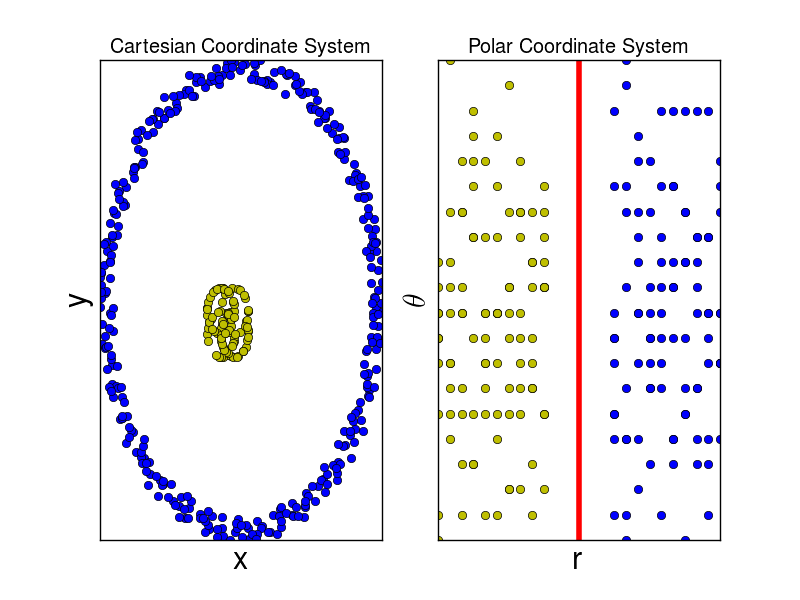
\includegraphics[width=0.7\textwidth]{./images/chapter3/representation_dependency.png}
  \caption[Παράδειγμα διαφορετικών αναπαραστάσεων των δεδομένων]{Παράδειγμα διαφορετικών αναπαραστάσεων των δεδομένων}
  \label{fig:representation_dependency}
\end{figure}

Ένα απλό και κατανοητό παράδειγμα, το οποίο δείχνει την εξάρτηση της επίδοσης ενός
αλγορίθμου ML, από την μορφή της αναπαράστασης που του δίνεται, φαίνεται στο
\autoref{fig:representation_dependency}. Έστω ότι θέλουμε να
διαχωρίσουμε τα δεδομένα μας σε δύο κλάσεις, χαράζοντας μία ευθεία
μεταξύ τους. Αν αναπαραστήσουμε τα δεδομένα στο Καρτεσιανό σύστημα συντεταγμένων (αριστερό διάγραμμα),
τότε η επίλυση του προβλήματος είναι αδύνατη αφού δεν υπαρχει καμία ευθεία
που να διαχωρίζει τις δύο κλάσεις. Ωστόσο, αν αναπαραστήσουμε τα δεδομένα
στο Πολικό σύστημα συντεταγμένων (δεξί διάγραμμα), τότε το πρόβλημα λύνεται
εύκολα, χαράζοντας μία κάθετη ευθεία, με $r  = a, a \in [r1, r2]$.

Σε πληθώρα προβλημάτων τεχνητής νοημοσύνης, η επιλογή κατάλληλων χαρακτηριστικών
είναι δύσκολο και χρονοβόρο έργο. Έστω για παράδειγμα ότι θέλουμε να αναγνωρίσουμε
πρόσωπα σε εικόνες. Ένα χαρακτηριστικό θα μπορούσε να είναι τα μάτια. Δυστυχώς όμως,
η αναγνώριση ματιών είναι και αυτή ένα δύσκολο πρόβλημα, αφού δεν μπορεί να
περιγραφεί πάντα επακριβώς έχοντας σαν δεδομένα τις τιμές των pixel της εικόνας.
Η γεωμετρική, για παράδειγμα, μορφή των ματιών σε μία εικόνα λήψης εξαρτάται από την
γωνία λήψης, τον φωτισμό, κτλ.


%\section{Εισαγωγή στην Επιστήμη της Μηχανικής Μάθησης}
\label{sec:theory_ml}

Τα τελευταία χρόνια, ο κλάδος της Τεχνιτής Νοημοσύνης είναι ένας από τους πιο ραγδαία
αναπτυσσόμενους κλάδους της επιστήμης της πληροφορικής με τεράστιο
ερευνητικό και πρακτικό ενδιαφέρον; διαιρείται σε δύο υπο\_\_\_; την \emph{συμβολική τεχνιτή
νοημοσύνη} και την \emph{υποσυμβολική τεχνητή νοημοσύνη}. Η πρώτη προσπαθεί να
επιλύσει τα προβλήματα χρησιμοποιώντας αλγοριθμικές διαδικασίες, δηλαδή
σύμβολα και λογικούς κανόνες, ενώ η δεύτερη προσπαθεί να αναπαράγει την
ανθρώπινη "ευφυία" μέσα από την χρήση αριθμητικών μοντέλων
που με την σύνθεσή τους προσομοιώνουν την λειτουργία του ανθρώπινου εγκεφάλου
(υπολογιστική νοημοσύνη).
Η ικανότητα ενός νοούμενου (AI) συστήματος, να αποκτά από μόνο του γνώση,
εξάγοντας πρότυπα ή/και χαρακτηριστικά σημεία από τα δεδομένα,
είναι γνωστή ώς \emph{Μηχανική Μάθηση} (ML).
Η εισαγωγή του κλάδου του ML στην επιστήμη των υπολογιστών,
επέτρεψε στους υπολογιστές να μπορούν να αντιμετωπίσουν προβλήματα που εμπλέκουν
την αντίληψη για τον πραγματικό κόσμο και να πέρνουν υποκειμενικές αποφάσεις.

Η χρησιμοποίηση αλγορίθμων ML, επιτρέπουν σε συστήματα AI
να προσαρμόζονται εύκολα σε καινούργια έργα, με ελάχιστη επέμβαση από τον άνθρωπο.
Για παράδειγμα, ένα Νευρωνικό Δίκτυο που έχει εκπεδευτεί να αναγνωρίζει γάτους σε εικόνες,
δεν απαιτεί να σχεδιαστεί και να εκπαιδευτεί από το μηδέν για να έχει την ικανότητα
να αναγνωρίζει και σκύλους.

Πολλά προβλήματα, ενώ μέχρι και πριν μία πεντα-ετία λύνονταν με
"χειρόγραφη", προγραμματισμένη από τον άνθρωπο, γνώση
(hand-written feature extraction), σήμερα χρησιμοποιούνται
αλγόριθμοι ML για την επίλυσή τους. Πιο κάτω παρατίθενται μερικά
παραδείγματα:
\begin{itemize}
  \item{Αναγνώριση ομιλίας - Speech Recognition}
  \item{Μηχανική όραση - Computer Vision}
  \begin{itemize}
    \item{Αναγνώριση αντικειμένων σε εικόνες - Object Recognition}
    \item{Αναγνώριση και εντοπισμός της θέσης αντικειμένων σε εικόνες - Object Detection}
  \end{itemize}
  \item{Αναγνώριση ηλεκτρονικών επιθέσεων στο διαδίκτυο - Cyberattack detection}
  \item{Επεξεργασία φυσικής γλώσσας - Natural Language Processing}
  \begin{itemize}
    \item{Κατανόηση της φυσικής γλώσσας του ανθρώπου - Natural Language Understanding}
    \item{Μοντελοποίηση και χρησιμοποίηση της φυσικής γλώσσας του ανθρώπου από μηχανές - Natural Language Generation}
  \end{itemize}
  \item{Μηχανές αναζήτησης}
\end{itemize}

Η μορφή της αναπαράστασης των δεδομένων αποτελεί σημαντικό παράγοντα στην
απόδοση των αλγορίθμων ML. Μία αναπαράσταση αποτελείτε από χαραχτηριστικά (features).
Για παράδειγμα, ένα χρήσιμο χαρακτηριστικό, στην ταυτοποίηση ομιλιτή, από δεδομένα ήχου,
είναι η εκτίμηση του μεγέθους της φωνητικής έκτασης του ομιλιτή.
Έτσι, πολλά προβλήματα τεχνητής νοημοσύνης, μπορούν να λυθούν
με κατάλληλη σχεδίαση και επιλογή των χαρακτηριστικών, για το συγκεκριμένο
πρόβλημα. Το σύνολο των χαρακτηριστικών αυτών αποτελεί την αναπαράσταση των δεδομένων,
σε ένα πιο υψηλό και αφαιρετικό επίπεδο αντίληψης για τους υπολογιστές, η οποία
στην συνέχεια δίνεται σαν είσοδος σε έναν απλό ML αλγόριθμο, ο οποίος έχει
μάθει να αντιστοιχεί την αναπαράσταση των δεδομένων στην επιθυμητή έξοδο.


\section{Deep Neural Networks}
\label{sec:theory_dnn}

The computations involved in producing an output from an input can be represented by a flow graph: a flow graph is a graph representing a computation, in which each node represents an elementary computation and a value (the result of the computation, applied to the values at the children of that node). Consider the set of computations allowed in each node and possible graph structures and this defines a family of functions. Input nodes have no children. Output nodes have no parents.

\section{Νευρωνικά Δίκτυα Συνέλιξης}
\label{sec:theory_cnn}

Μέχρι τώρα μιλήσαμε για τα πολυεπίπεδα νευρωνικά δίκτυα και την γενικότερη
λειτουργία τους. Σε αυτό το υποκεφάλαιο θα μιλήσουμε για συγκεκριμένα μοντέλα
πολυεπίπεδων νευρωνικών δικτύων και πιο συγκεκριμένα για τα
\emph{νευρωνικά Δίκτυα Συνέλιξης}. Τα συγκεκριμένα μοντέλα χρησιμοποιούνται
σήμερα κυρίως στα προβλήματα της αναγνώρισης και εντοπισμού αντικειμένων
σε εικόνες.

Ο τρόπος λειτουργίας τους είναι όμοιος με αυτόν που παρουσιάστηκε στο
\autoref{sec:dnn}; αποτελούνται από πολλά επίπεδα, όπου το κάθε επίπεδο αποτελείται
από έναν αριθμό νευρώνων οι οποίοι έχουν σαν παραμέτρους εκμάθησης τα βάρη ($w_{\jmath}^{\imath}$) τους
και την τιμή πόλωσης ($b^{\imath}$).
Κάθε νευρώνας δέχεται ένα σήμα εισόδου , εφαρμόζει μία πράξη εσωτερικού γινομένου σε αυτό,
και προαιρετικά περνάει το αποτέλεσμα από μία μη γραμμική συνάρτηση.
Το τελευταίο επίπεδο των CNN είναι ένας πλήρες συνδεδεμένο επίπεδο και έχει μία
συνάρτηση σφάλματος.
Η διαφορά των μοντέλων CNN από τα κλασσικά ANN είναι ότι θεωρούν για δεδομένα εισόδου
εικόνες.

Αυτό που καταφέρνουν να κάνουν τα CNN είναι να μοντελοποιήσουν μικρά
κομμάτια πληροφορίας τα οποία στην συνέχεια ενώνονται για να δημιουργήσουν
υψηλότερου επιπέδου πληροφορία. Αν για παράδειγμα παρατηρήσουμε την λειτουργία
ενός μοντέλου CNN, το πρώτο επίπεδο προσπαθεί να εντοπίσει ακμές, το δεύτερο
επίπεδο και παίρνοντας την πληροφορία αυτή των ακμών προσπαθεί να εντοπίσει περιγράμματα,
κτλ.


Σε κάθε πίξελ της εικόνας αντιστοιχούν 3 τιμές (RGB) και άρα η είσοδος σε ένα
CNN έχει τρεις διαστάσεις όπως φαίνεται και στο \autoref{fig:cnn_1}.
Για παράδειγμα ένα CNN το οποίο έχει σχεδιαστεί να δέχεται σαν είσοδο εικόνες ανάλυσης $80\times60$
έχει επίπεδο εισόδου διαστάσεων $80\times60\times3$.

\begin{figure}[!ht]
  \centering
  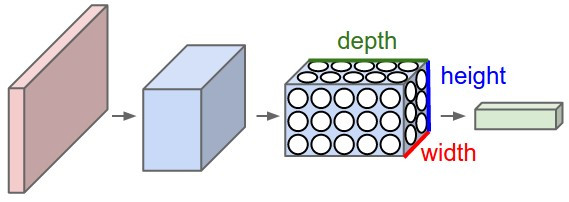
\includegraphics[width=0.8\textwidth]{./images/chapter3/cnn.jpg}
  \caption[Τρισδιάστατη κατανομή των νευρώνων στα CNN]{Τρισδιάστατη κατανομή των νευρώνων στα CNN}
  \label{fig:cnn_1}
\end{figure}

Κάθε επίπεδο ενός CNN παίρνει σαν είσοδο μία μορφή όγκου την οποία
και μετασχηματίζει σε μία άλλη μορφή όγκου.

Οι τρεις βασικοί τύποι επιπέδων που χρησιμοποιούνται σε αρχιτεκτονικές CNN είναι:
\begin{itemize}
  \item{Επίπεδο Συνέλιξης - Convolutional Layer (CONV)}
  \item{Επίπεδο Υπό-δειγματοληψίας- Pooling Layer (POOL)}
  \item{Πλήρη Συνδεδεμένο Επίπεδο - Fully-Connected Layer (FC)}
\end{itemize}
Μία σημαντική παρατήρηση είναι ότι τα επίπεδα CONV και FC έχουν παραμέτρους, δηλαδή
βάρη και τιμή πόλωσης των νευρώνων, ενώ τα επίπεδα POOL εκτελούν λειτουργία
δειγματοληψίας στα δεδομένα εισόδου τους.


\subsection{Επίπεδο Συνέλιξης}

Τα επίπεδα συνέλιξης είναι ο πυρήνας των μοντέλων CNN. Οι παράμετροι ενός
επιπέδου CONV είναι μία σειρά από δισδιάστατα φίλτρα τα οποία όμως εκτείνονται
σε όλο το σε όλο το βάθος του όγκου εισόδου. Το βάθος των φίλτρων αυτών
ισούται με το βάθος του όγκου στην είσοδο.


Όπως αναφέραμε και προηγουμένως, τα επίπεδα CONV εφαρμόζουν πράξη συνέλιξης πάνω στα
δεδομένα εισόδου. Αυτό επηρεάζει στην δομή των "τοπικών" διασυνδέσεων.
Στο παράδειγμα του σχήματος \ref{fig:cnn_2} βλέπουμε πως ο κάθε νευρώνας
του επιπέδου συνέλιξης συνδέεται με μία περιοχή του όγκου στην είσοδό του.

\begin{figure}[!ht]
  \centering
  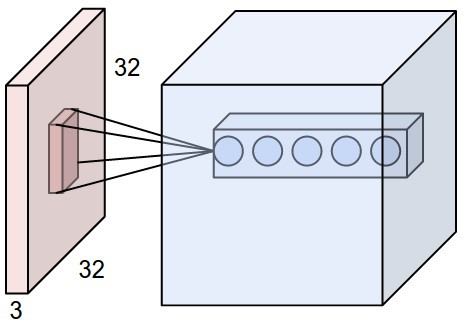
\includegraphics[width=0.4\textwidth]{./images/chapter3/cnn_2.jpg}
  \caption[%
    Παράδειγμα διασύνδεσης τρισδιάστατης εισόδου με την τρισδιάστατη δομή των
    νευρόνων ενός επιπέδου συνέλιξης (CONV)]{%
    Παράδειγμα διασύνδεσης τρισδιάστατης εισόδου με την τρισδιάστατη δομή των
    νευρόνων ενός επιπέδου συνέλιξης (CONV)}
  \label{fig:cnn_2}
\end{figure}

Η συνέλιξη ενός φίλτρου με τον τον όγκο εισόδου παράγει έναν \emph{χάρτη ενεργοποίησης (activation map)},
με τον τρόπο που φαίνεται στο \autoref{fig:cnn_activation_map}. Στο παράδειγμα αυτό
εφαρμόζεται φίλτρο διαστάσεων $5\times5\times3$ σε έναν όγκο $32\times32\times3$ και παράγεται
ένας χάρτης ενεργοποίησης διαστάσεων $28\times28\times1$.

\begin{figure}[!ht]
  \centering
  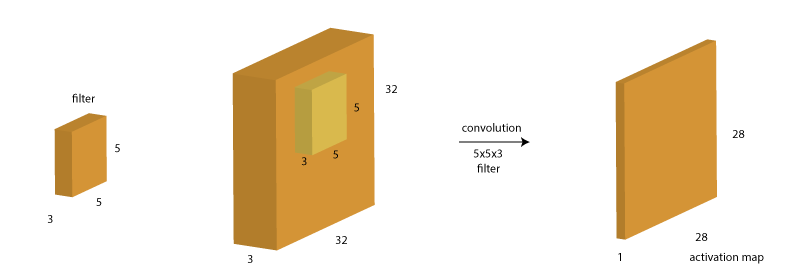
\includegraphics[width=1\textwidth]{./images/chapter3/cnn_activation_map.png}
  \caption[Συνέλιξη φίλτρου ενός επιπέδου συνέλιξης με τον όγκο εισόδου και παραγωγή ενός χάρτη ενεργοποίησης]{Συνέλιξη φίλτρου ενός επιπέδου συνέλιξης με τον όγκο εισόδου και παραγωγή ενός χάρτη ενεργοποίησης}
  \label{fig:cnn_activation_map}
\end{figure}

Η μείωση των διαστάσεων μήκους και πλάτους από $32\times32$ σε $28\times28$ οφείλεται στον τρόπο με τον οποίο
εκτελείται η πράξη της συνέλιξης των φίλτρων με τον όγκο εισόδου  (\autoref{fig:cnn_conv}).
Οι διαστάσεις του όγκου εξόδου, έχοντας σαν είσοδο όγκο διαστάσεων $N \times N \times d$ και φίλτρων $F \times F \times d$ υπολογίζονται, στην απλούστερη περίπτωση με βάση την σχέση
\begin{equation*}
  outsize = (N-F) + 1
\end{equation*}


\begin{figure}[!ht]
  \centering
  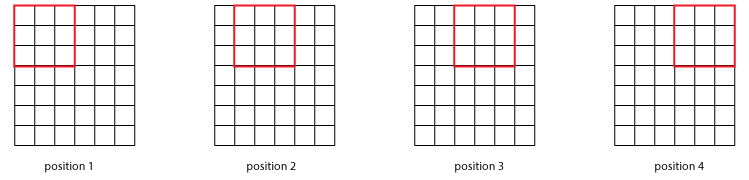
\includegraphics[width=1\textwidth]{./images/chapter3/cnn_conv.png}
  \caption[Διαδικασία Συνέλιξης]{Διαδικασία Συνέλιξης}
  \label{fig:cnn_conv}
\end{figure}

Η τιμή του βάθους του όγκου στην έξοδο ενός επιπέδου CONV αντιστοιχεί στον αριθμό των φίλτρων που
εφαρμόζονται στον όγκο εισόδου. Δηλαδή ο αριθμός των χαρτών ενεργοποίησης
αντιστοιχεί στον αριθμό των φίλτρων. Αν για παράδειγμα ο όγκος εισόδου είναι
διαστάσεων $32\times\32\times3$ και εφαρμόσουμε δέκα φίλτρα συνέλιξης διαστάσεων $5\times5\times3$,
ο όγκος εξόδου θα είναι διαστάσεων $28\times28\times3$ \autoref{fig:cnn_num_filters}.
Ο αριθμός των φίλτρων είναι μία παράμετρος, ή καλύτερα \emph{υπερ-παράμετρος} των επιπέδων συνέλιξης.

\begin{figure}[!ht]
  \centering
  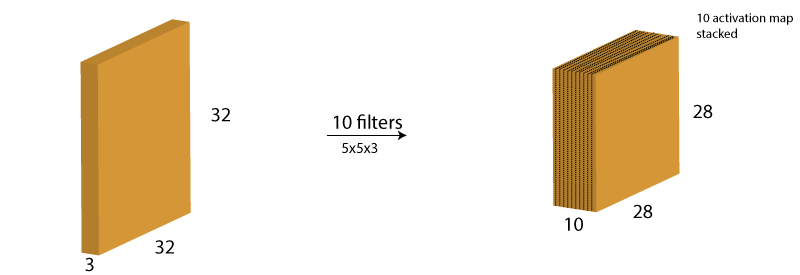
\includegraphics[width=1\textwidth]{./images/chapter3/cnn_num_filters.png}
  \caption[Αντιστοιχία του αριθμού των φίλτρων ενός επιπέδου συνέλιξης με το βάθος του όγκου στην έξοδο]{Αντιστοιχία του αριθμού των φίλτρων ενός επιπέδου συνέλιξης με το βάθος του όγκου στην έξοδο}
  \label{fig:cnn_num_filters}
\end{figure}

Ωστόσο, το βήμα μετατόπισης (stride) του φίλτρου πάνω στην είσοδο είναι και αυτό
μία υπέρ-παράμετρος (hyperparameter) των επιπέδων συνέλιξης.
Χρησιμοποιώντας βήμα μετατόπισης (S) διάφορο της μονάδας καταλήγουμε στην πιο κάτω
εξίσωση για τον υπολογισμό του όγκου εξόδου:
\begin{equation*}
  outsize = (N-F)/S + 1
\end{equation*}

Ένα πρόβλημα που εμφανίζεται στην περίπτωση των μοντέλων CNN με μεγάλο αριθμό
κρυφών επιπέδων είναι η γρήγορη μείωση των διαστάσεων μήκους και πλάτους του
όγκου, το οποίο είναι αποτέλεσμα της διαδοχική εφαρμογή πράξεων συνέλιξης (\autoref{fig:cnn_shrunk}).

\begin{figure}[!ht]
  \centering
  
\includegraphics[width=1\textwidth]{./images/chapter3/cnn_shrunk.png}
  \caption[Διαδοχικές εφαρμογές του τελεστή συνέλιξης προκαλούν μείωση των διαστάσεων μήκους και πλάτους του όγκου]{Διαδοχικές εφαρμογές του τελεστή συνέλιξης προκαλούν μείωση των διαστάσεων μήκους και πλάτους του όγκου}
  \label{fig:cnn_shrunk}
\end{figure}

Αυτή η συμπεριφορά είναι ανεπιθύμητη αφού περιορίζει και τις διαστάσεις των φίλτρων
που μπορούμε να χρησιμοποιήσουμε σε κάθε επίπεδο CONV. Η χρήση φίλτρων μεγάλων
διαστάσεων φέρει σαν αποτέλεσμα την γρήγορη μείωση των διαστάσεων του όγκου.

Για να αποτρέψουμε αυτή την συμπεριφορά μπορούμε να επεκτείνουμε τις διαστάσεις
μήκους και πλάτους, προσθέτοντας μηδενικά στα σύνορα του όγκου εισόδου του
εκάστοτε επιπέδου CONV. Η διαδικασία αυτή ονομάζεται
\emph{zero-padding} και φαίνεται στο \autoref{fig:cnn_zero_padding}.
\begin{figure}[!ht]
  \centering
  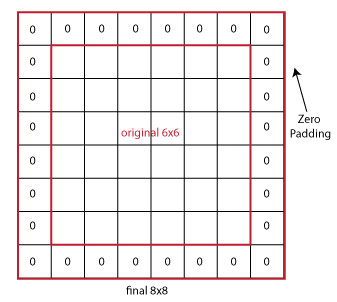
\includegraphics[width=0.6\textwidth]{./images/chapter3/cnn_zero_padding.png}
  \caption[Zero Padding]{Zero Padding}
  \label{fig:cnn_zero_padding}
\end{figure}
Το μέγεθος του συνόρου που προστίθεται είναι η τρίτη υπέρ-παράμετρος ενός
επιπέδου συνέλιξης.

Με την εισαγωγή της υπέρ-παραμέτρου zero-padding η εξίσωση υπολογισμού του όγκου
εξόδου έχει την μορφή:
\begin{equation*}
  outsize = (N - F + 2P)/S + 1
\end{equation*}

Συνοψίζοντας, ένα επίπεδο συνέλιξης έχει τα εξής χαρακτηριστικά:
\begin{itemize}
  \item{Διαστάσεις όγκου εισόδου: $W_{1} \times H_{1} \times D_{1}$}
  \item{Hyperparameters:}
    \begin{itemize}
      \item{K: Αριθμός φίλτρων}
      \item{F: Μέγεθος του φίλτρου ($F \times F$)}
      \item{S: Βήμα μετατόπισης}
      \item{P: Ποσότητα zero-padding}
    \end{itemize}
  \item{Διαστάσεις όγκου εξόδου: $W_{2} \times H_{2} \times D_{2}$, $D_{2} = K$} όπου:
    \begin{itemize}
      \item{$W_{2} = (W_{1} - F)/S + 1$}
      \item{$H_{2} = (H_{1} - F)/S + 1$}
      \item{$D_{2} = D_{1}$}
    \end{itemize}
\end{itemize}


\subsection{Επίπεδο Υπό-δειγματοληψίας - Pooling layer}

Συνήθως τα επίπεδα υπό-δειγματοληψίας προστίθενται στο δίκτυο, μεταξύ διαδοχικών
επιπέδων συνέλιξης. Η λειτουργία τους είναι να μειώσουν τις χωρικές
διαστάσεις των αναπαραστάσεων, μειώνοντας έτσι τον αριθμό των
παραμέτρων και άρα τους υπολογισμούς που γίνονται στο νευρωνικό δίκτυο
(\autoref{fig:cnn_pool}).

\begin{figure}[!ht]
  \centering
  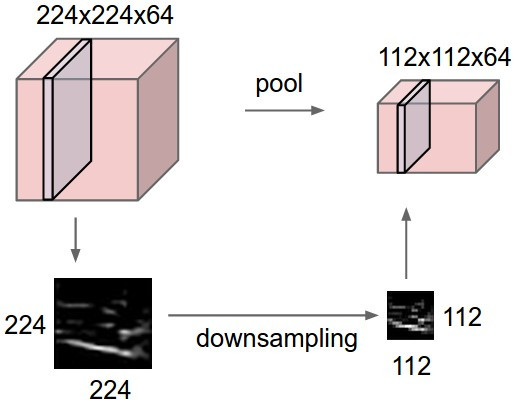
\includegraphics[width=0.6\textwidth]{./images/chapter3/cnn_pool.jpg}
  \caption[Επίπεδο Υποδειγματοληψίας - Pooling layer]{Επίπεδο Υπό-δειγματοληψίας - Pooling layer}
  \label{fig:cnn_pool}
\end{figure}
Ενεργεί δηλαδή σαν μία συνάρτηση υπό-δειγματοληψίας.
Πιθανές συναρτήσεις υπό-δειγματοληψίας είναι οι συναρτήσεις \emph{max, average και L2-Norm}

Στο \autoref{fig:cnn_pool_max} βλέπουμε το αποτέλεσμα της εφαρμογή της συνάρτησης
δειγματοληψίας $max(\vec{v})$ πάνω σε ένα πλέγμα διαστάσεων $4 \times 4$.

\begin{figure}[!ht]
  \centering
  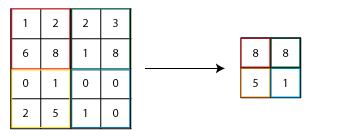
\includegraphics[width=0.6\textwidth]{./images/chapter3/cnn_pool_max.png}
  \caption[Συνάρτηση υπό-δειγματοληψίας Max - Max Pooling]{Συνάρτησης υποδειγματοληψίας Max - Max Pooling}
  \label{fig:cnn_pool_max}
\end{figure}

Τα χαρακτηριστικά των συναρτήσεων υπό-δειγματοληψίας είναι:
\begin{itemize}
  \item{Διαστάσεις όγκου εισόδου: $W_{1} \times H_{1} \times D_{1}$}
  \item{Hyperparameters:}
    \begin{itemize}
      \item{F: Χωρική τους έκταση ($F \times F$)}
      \item{S: Βήμα μετατόπισης}
    \end{itemize}
  \item{Διαστάσεις όγκου εξόδου: $W_{2} \times H_{2} \times D_{2}$, $D_{2} = K$} όπου:
    \begin{itemize}
      \item{$W_{2} = (W_{1} - F)/S + 1$}
      \item{$H_{2} = (H_{1} - F)/S + 1$}
      \item{$D_{2} = D_{1}$}
    \end{itemize}
\end{itemize}


\subsection{Πλήρως Συνδεδεμένο Επίπεδο - Fully-connected layer}

Ένα πλήρως συνδεδεμένο επίπεδο συνδέεται με όλους τους νευρώνες στο
προηγούμενο επίπεδο, όπως γίνεται στα απλά μοντέλα NN (Πολυεπίπεδος Perceptron),

Συνήθως το τελευταίο επίπεδο σε ένα CNN είναι πλήρως συνδεδεμένο και πιο
συγκεκριμένα έχει τόσους νευρώνες όσες και οι κλάσεις της πρόβλεψης. Για
παράδειγμα, ένα CNN που χρησιμοποιείται για αναγνώριση αντικειμένων σε
εικόνες CIFAR-10 έχει το τελευταίο επίπεδο του πλήρως συνδεδεμένο και
αποτελείται από 10 νευρώνες.

\section{Εφαρμογές Νευρωνκών Δικτύων Συνέλιξης στην Αναγνώριση Αντικειμένων στον Χώρο}
\label{sec:theory_object_recognition}


